\begin{frame}{Classical Feature Extraction}
\begin{itemize}
    \item \textbf{Problem:} Our images are too high-dimensional and flattening doesn't take advantage of innate local properties of images.
    \item \textbf{Solution:} Can our images be reduced to a set of features (also named a feature vector).
    \item In "classical" feature extraction, we rely on our human understanding of what a "good" local features is to decide what matters in a picture and what doesn't.
\end{itemize}
\end{frame}

\begin{frame}{Classical Feature Extraction}
    \begin{figure}
    \centering
    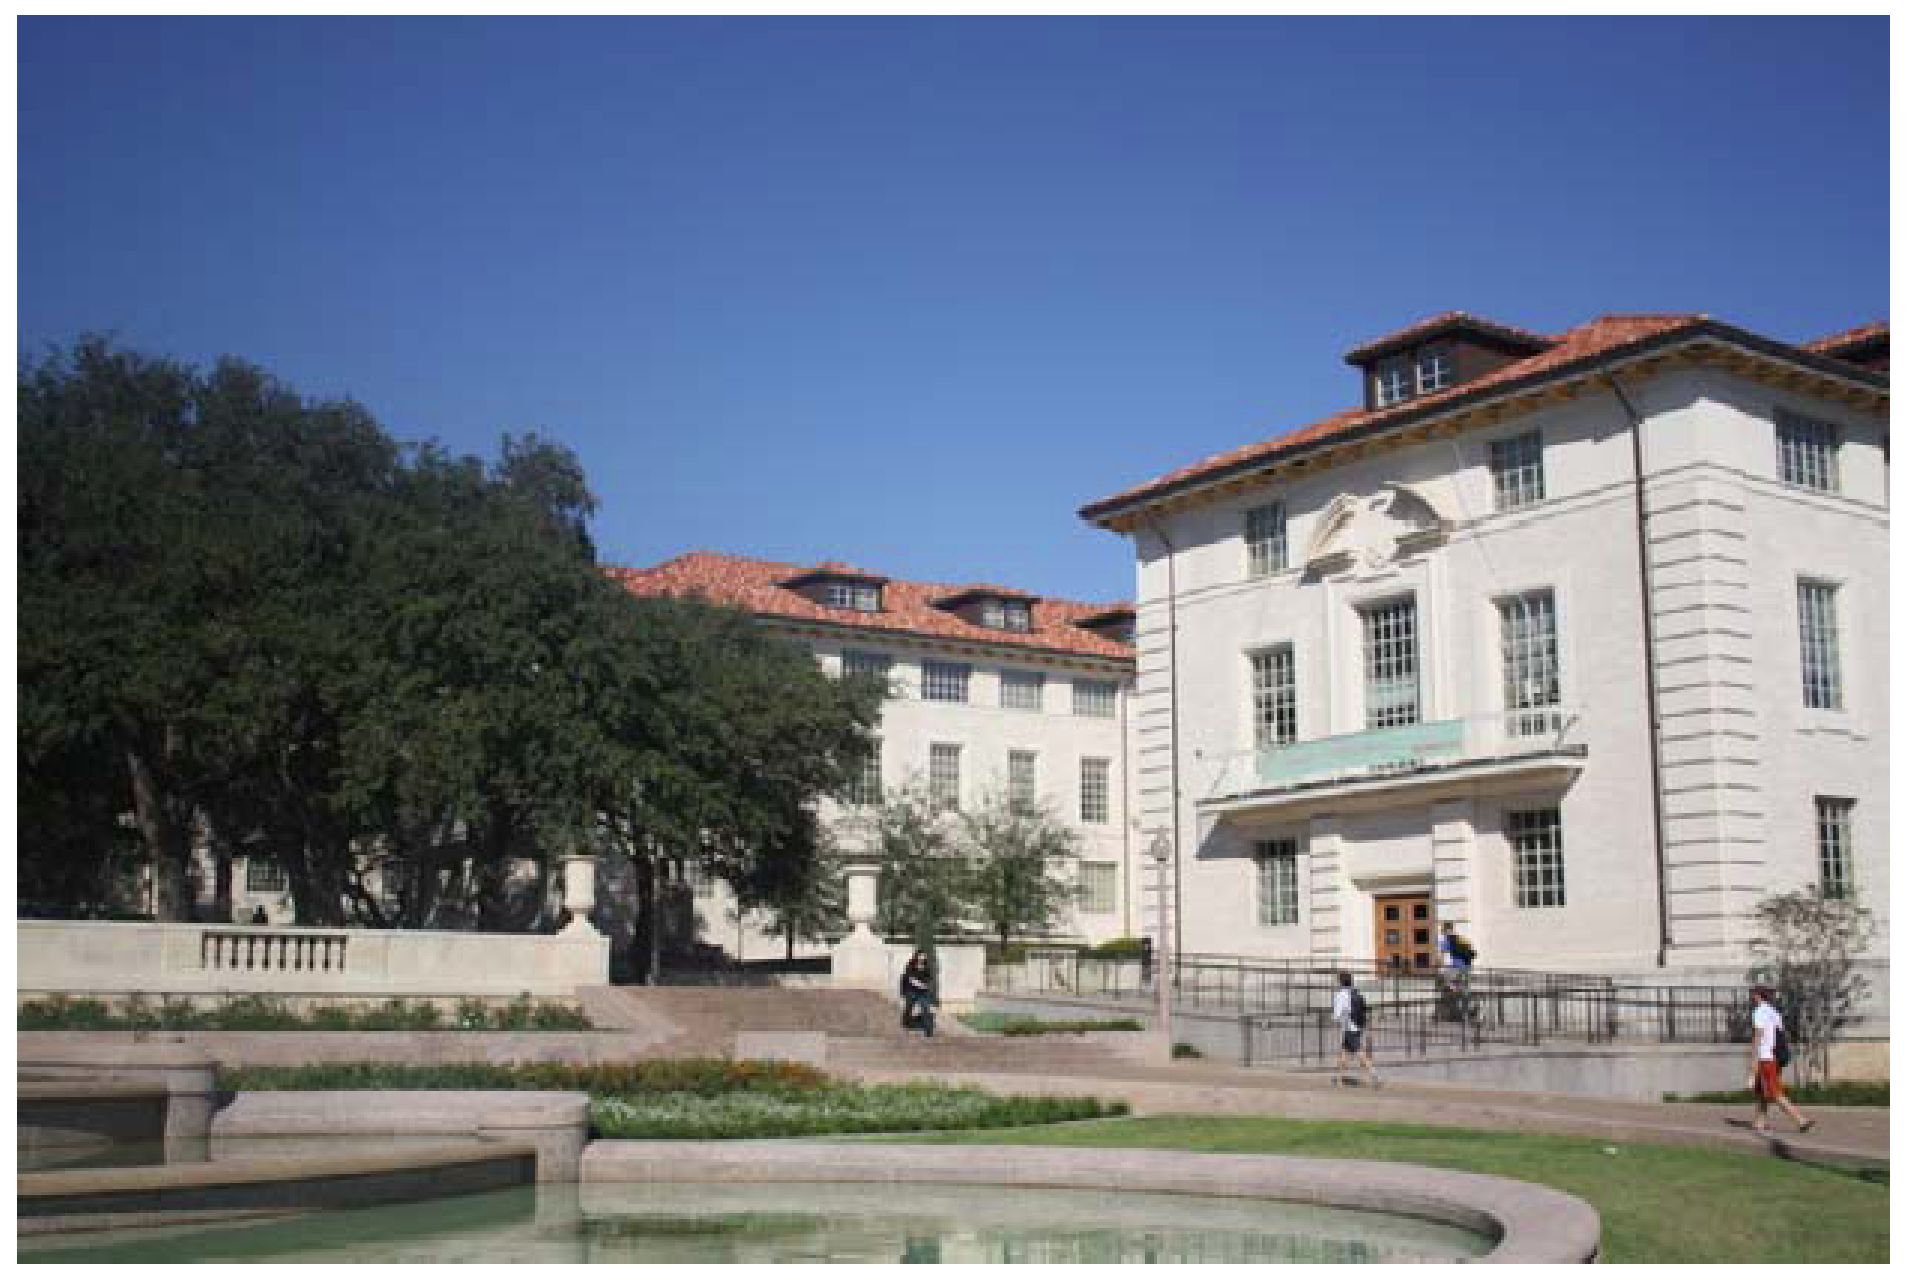
\includegraphics[width=0.8\textwidth]{img/house.png}
    \caption{Standard Image of a campus}
    \end{figure}
\end{frame}

\begin{frame}{Classical Feature Extraction}
    \begin{figure}
    \centering
    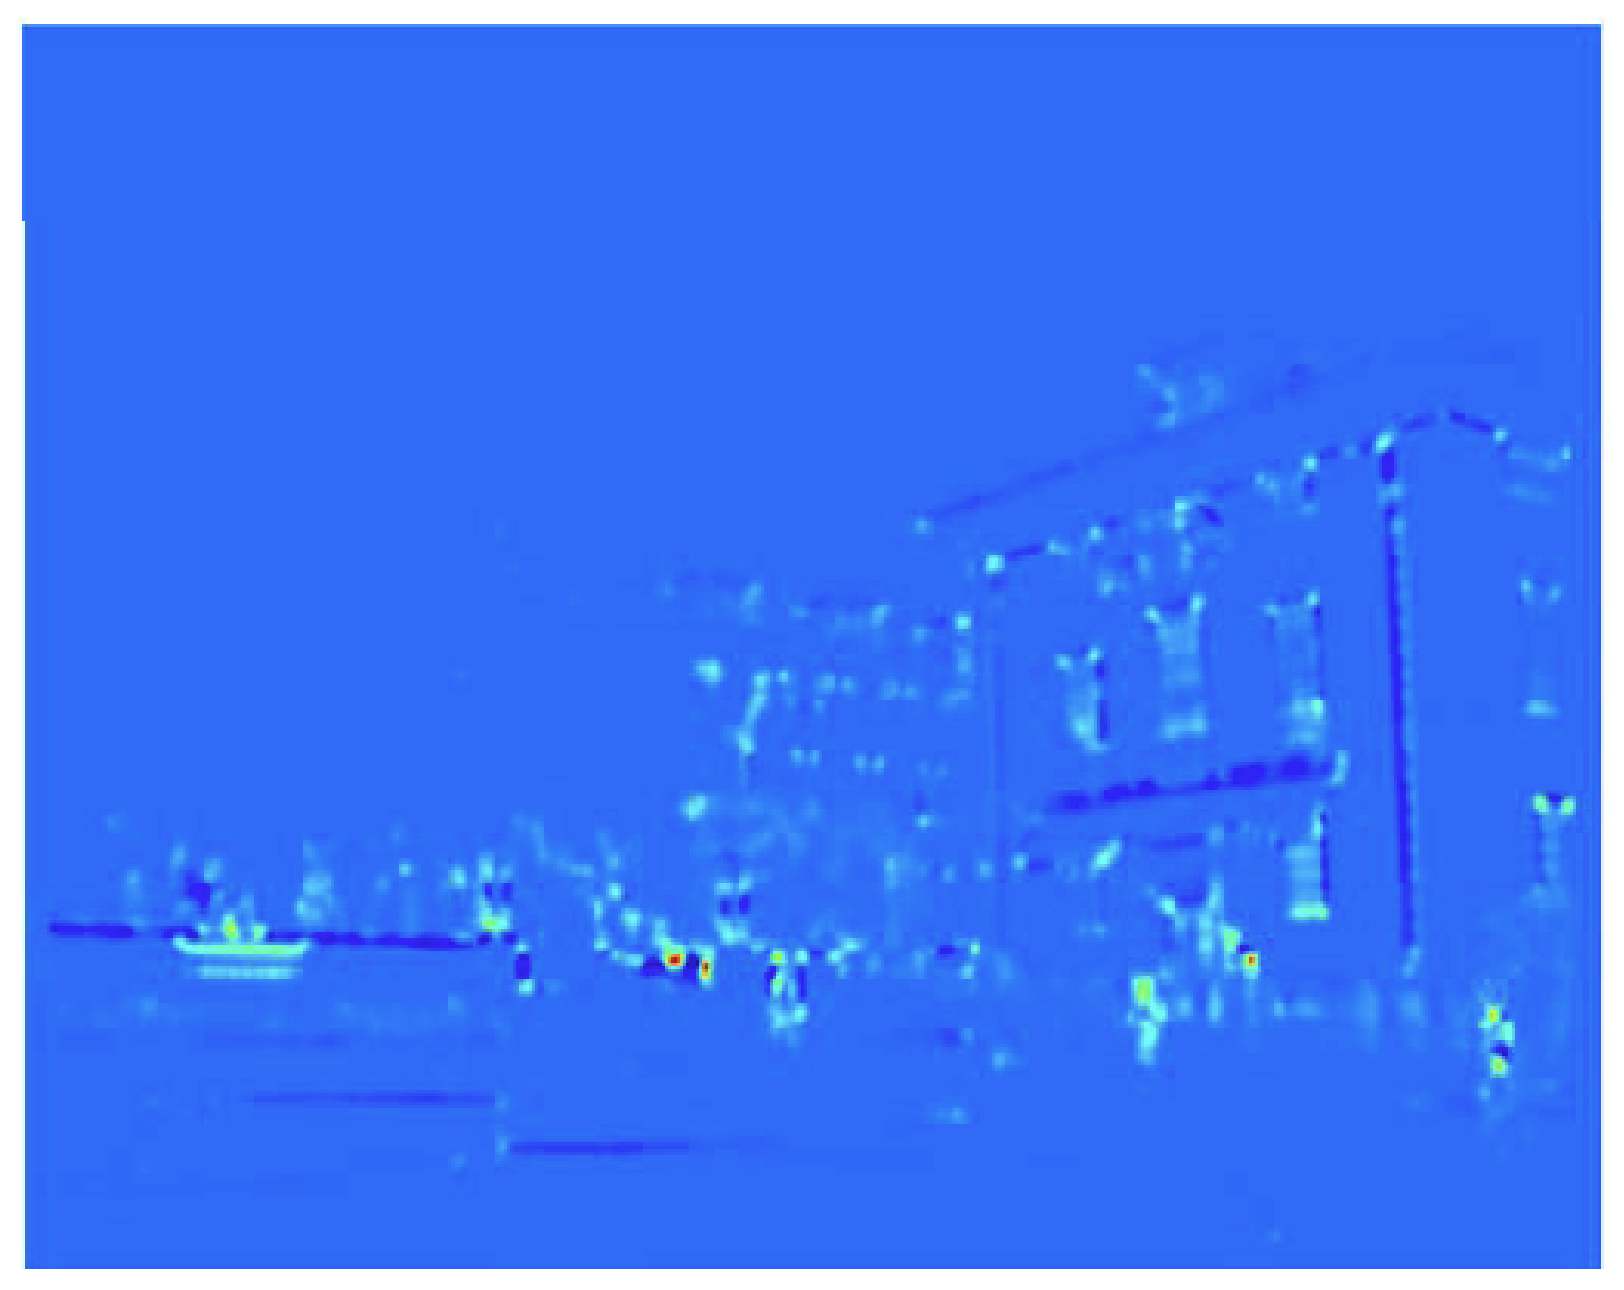
\includegraphics[width=0.6\textwidth]{img/cornernessheatmap.png}
    \caption{Search for parts of the image that have the most "cornerness"}
    \end{figure}
\end{frame}

\begin{frame}{Classical Feature Extraction}
    \begin{figure}
    \centering
    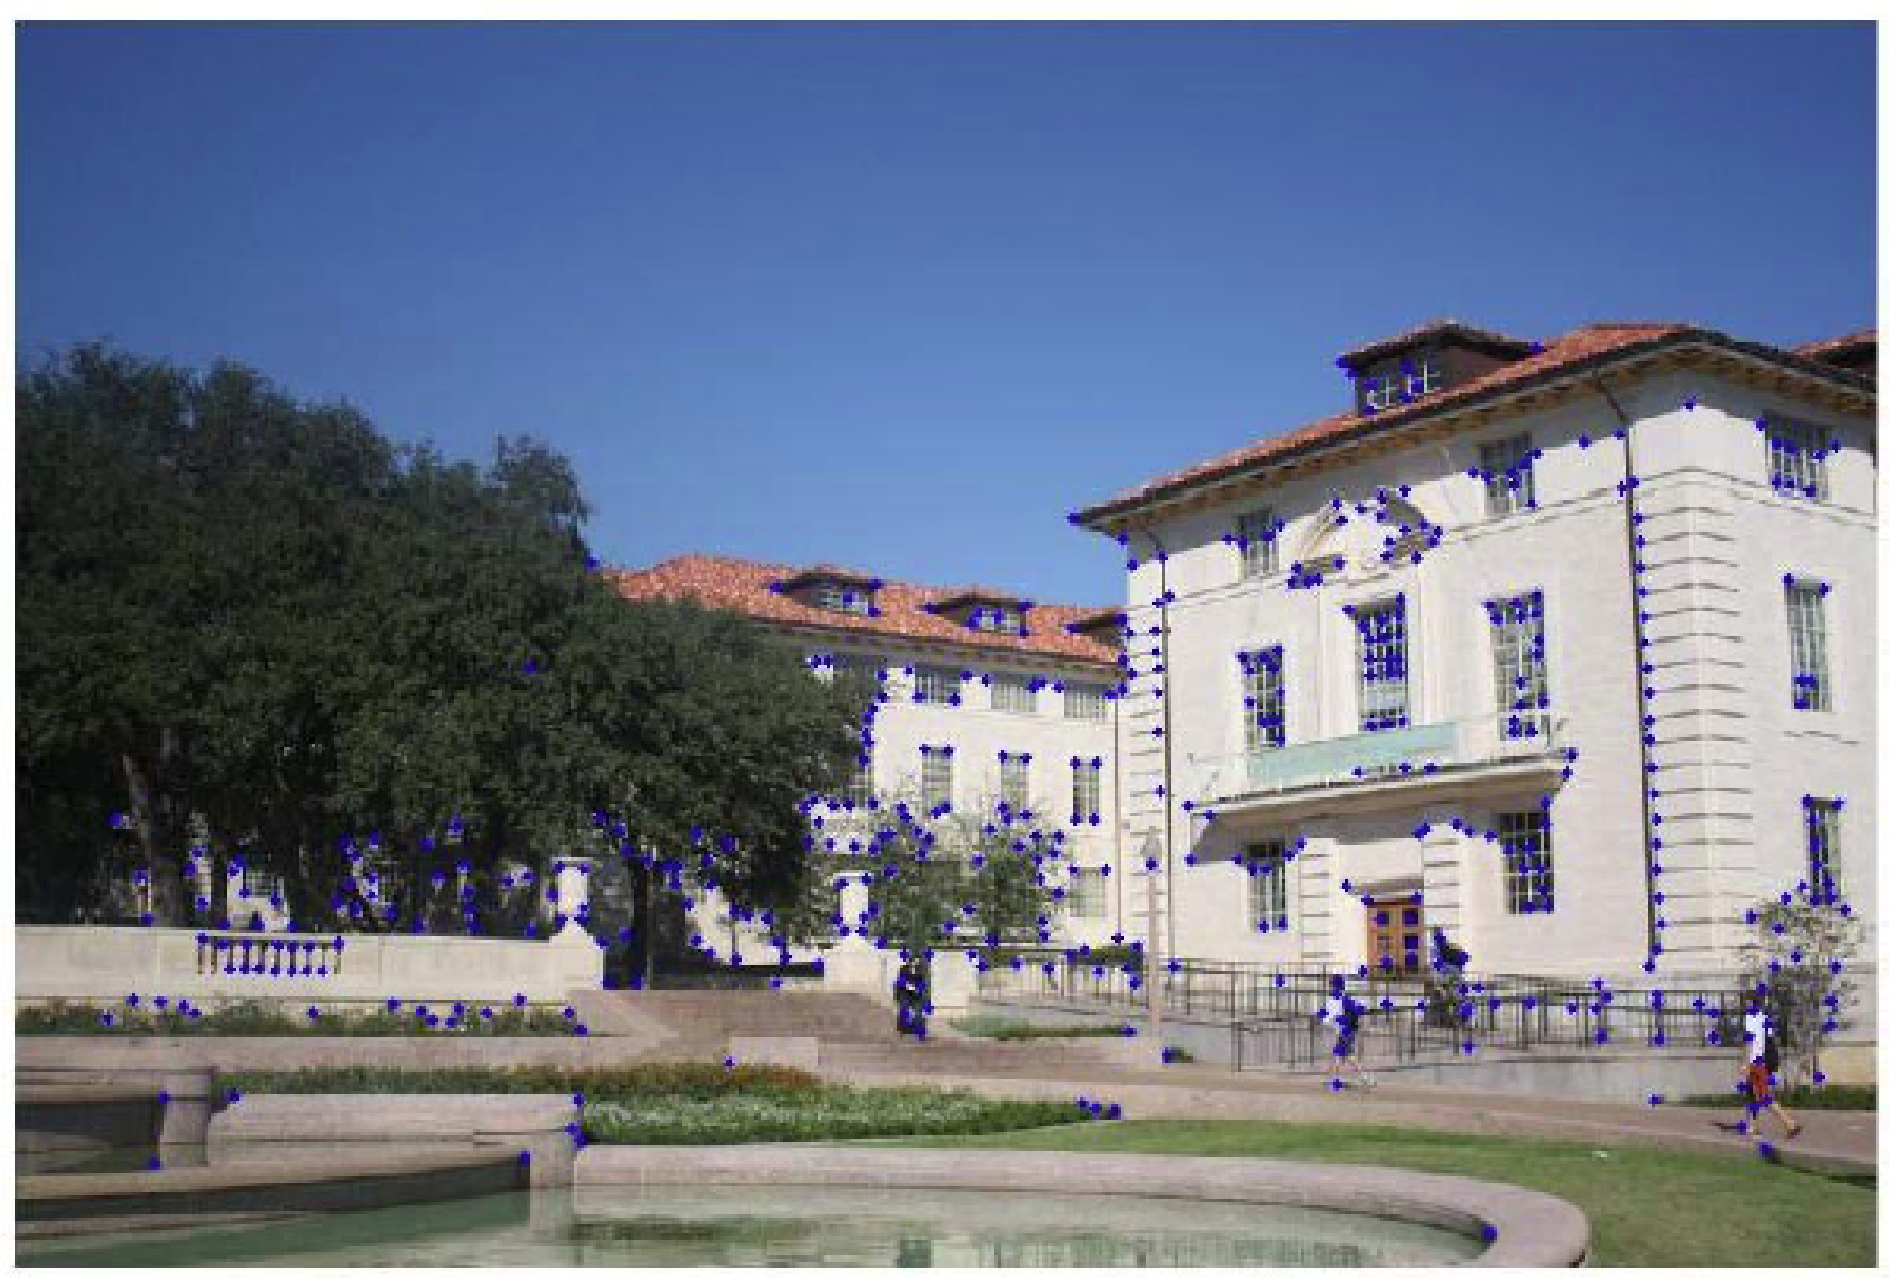
\includegraphics[width=0.8\textwidth]{img/houseinteresting.png}
    \caption{Based on our heatmap, extract points of interest}
    \end{figure}
\end{frame}

\begin{frame}{Classical Feature Extraction}
    \begin{figure}
    \centering
    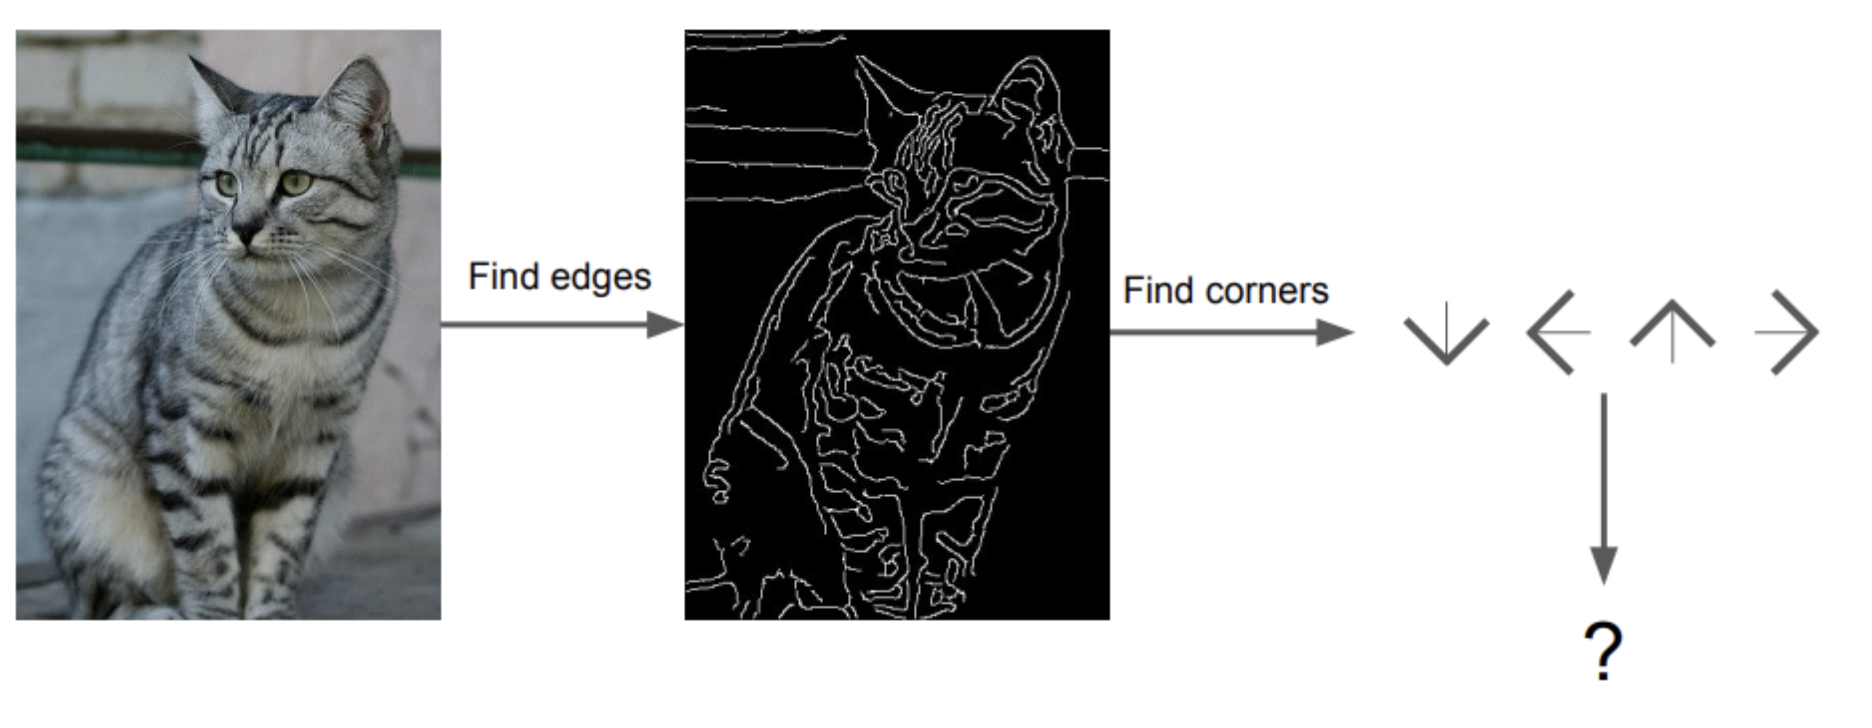
\includegraphics[width=0.8\textwidth]{img/edgecat.png}
    \caption{Extracting edges and corners can greatly reduce our input dimensionality while improving the model's understanding of local features}
    \end{figure}
\end{frame}